\chapter{Numerical Approach to the Thin-Structure Problem} \label{ch:Homogenisation}
\Cref{Graphs} explored the application of the tools that can be used to analyse singular-structure problems, and obtain information about their spectra.
The borderline case example will prove particularly useful here as it provides the effective problem for the thin-structure problem we will consider, in order to demonstrate the ability to estimate the spectrum of a 2-dimensional problem with that of a graph problem (as was claimed in \cref{Intro}).
In this chapter we will explore the spectrum of a thin-structure problem on a periodic domain, in the finite-frequency approximation as the length scales $N\rightarrow\infty$, $\epsilon\rightarrow0$ such that $\epsilon^{\alpha}N\rightarrow\gamma\in\bracs{0,\infty}$.
This will involve an introduction to the Finite Element Method and a derivation of the finite-dimensional approximation to the eigenvalue problem, followed by some analysis of the resulting problem.
Numerical results for the eigenfrequencies and eigenfunctions are presented for visualisation and to demonstrate that the spectra \say{fill-up} intervals in the positive real axis as $N\rightarrow\infty$, $\epsilon\rightarrow0$.

\section{The Thin-Structure Problem} \label{sec:ThinStrucProblem}
Suppose we have a periodic structure in $\reals^{2}$, whose periodic unit cell is the unit square.
The period cells themselves have microstructure of length scale $\epsilon$ and whose geometry composes a cross originating from the centre of the unit cell; whose arms are parallel to the co-ordinate axes, with width $\epsilon$.
Each arm of the cross meets the arc of a semi-circle of radius $\sqrt{\epsilon}$; with the straight edge of each semicircle lying along the edge of the unit cell, and with the midpoint of the straight edge sharing the midpoint of the (respective) periodic cell edge.
The unions of the cross and semicircles in each unit cell forms the domain.
Note that the radius of the semicircles and widths of the arms of the cross are chosen so that we shall be in the borderline case of vertex- and edge-volume decay.
This geometry is illustrated in \fref{HomogenisationProblemUnitCell}; and we denote these periodic unit cells by $P_{\epsilon}$.
Once again we seek to determine the spectrum of the operator $-\laplacian u$ on this domain, for $u\in\femSolSpace$, with zero-normal derivative boundary conditions imposed on the boundary.
\begin{figure}[b!]
	\centering
	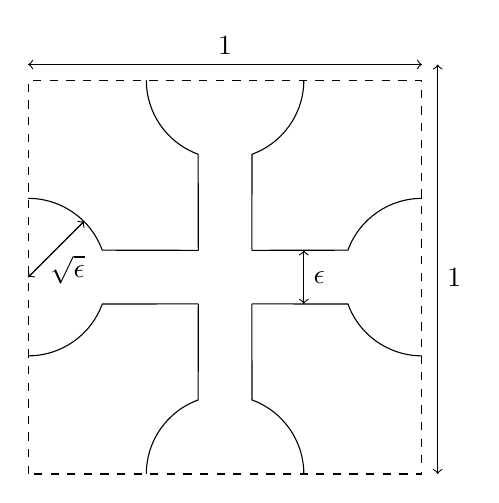
\begin{tikzpicture}
		\draw[dashed] (0,0) rectangle (5,5);
		\draw (0,3.5) arc (90:20:1) -- (2.16,2.84);
		\draw (0,1.5) arc (270:340:1) -- (2.16, 2.16);
		\draw (1.5,0) arc (180:110:1) -- (2.16, 2.16);
		\draw (3.5,0) arc (0:70:1) -- (2.84, 2.16);
		\draw (5,3.5) arc (90:160:1) -- (2.84, 2.84);
		\draw (5,1.5) arc (270:200:1) -- (2.84, 2.16);
		\draw (1.5,5) arc (180:250:1) -- (2.16, 2.84);
		\draw (3.5,5) arc (359.99:290:1) -- (2.84, 2.84);
		\node[anchor=west] at (3.5,2.5) {$\epsilon$};
		\draw[->] (3.5,2.16) -- (3.5,2.84);
		\draw[->] (3.5,2.84) -- (3.5,2.16);
		\draw[->] (0,2.5) -- (0.71,3.21);
		\draw[->] (0.71,3.21) -- (0,2.5);
		\node[anchor=north] at (0.5, 2.9) {$\sqrt{\epsilon}$};
		\draw[->] (0,5.2) -- (5,5.2);
		\draw[->] (5,5.2) -- (0,5.2);
		\node[anchor=south] at (2.5,5.2) {$1$};
		\draw[->] (5.2,5.2) -- (5.2,0);
		\draw[->] (5.2,0) -- (5.2,5.2);
		\node[anchor=west] at (5.2,2.5) {$1$};
		\end{tikzpicture}
	\caption{The unit cell of the periodic structure. The radius of the (semi-) circles is chosen so that the volume of the circles decays at the same rate as the volume of the tubes.\label{fig:HomogenisationProblemUnitCell}}
\end{figure} \newline

Setting up the finite-frequency approximation (\sref{FreqApproxes}), let $N\in\naturals$, and consider the domain $\homDomain_{\epsilon, N}\subset[0,N]^{2}$ formed from stacking $N^{2}$ translated copies of $P_{\epsilon}$ into a square. 
We divide the boundary $\partial\homDomain_{\epsilon, N}$ into two disjoint subsets:
\begin{align*}
	\perBoundary &:= \partial\homDomain_{\epsilon, N}\cap\bracs{\bracs{\set{0,N}\times[0,N]}\cup\bracs{[0,N]\times\set{0,N}}} \text{ and } \\
	\othBoundary &:= \partial\homDomain_{\epsilon, N}\setminus\perBoundary,
\end{align*} 
which are the interior boundary $\othBoundary$ which outlines the holes in the domain; and the periodic boundary $\perBoundary$ which comprises the semicircle straight-edges which have periodic boundary conditions imposed on them.
On $\homDomain_{\epsilon, N}$ we obtain the eigenvalue problem
\begin{subequations} \label{eq:HomProbFull}
	\begin{align} 
		-\laplacian u = \omega^{2}u &\quad \mathrm{on \:} \homDomain_{\epsilon, N} \label{eq:HomProbMain}\\
		\mathbf{n}\cdot\grad u = 0 &\quad \mathrm{on \:} \othBoundary \label{eq:HomProbNeumann}\\
		u \text{ is periodic across } &\quad \perBoundary.
	\end{align}
\end{subequations}

\section{Overview of the Finite Element Method} \label{sec:FEMSetup}
The geometry of the domain makes an analytic approach to the problem difficult, so we turn to numerical techniques to aid our analysis - in particular the Finite Element Method (FEM). 
The basis of the FEM is to write the boundary value problem \eref{HomProbFull} in the weak formulation, and then to solve the weak formulation on some finite-dimensional function space to obtain an approximate solution. 
The FEM has well-established theory, (in this report we follow \cite{johnson2012numerical}) and so we also provide statements of key convergence and error results. \newline

We first define a mesh for our domain $\homDomain_{\epsilon, N}$, which is a set of triangles (called mesh-elements or simply elements) $\eleSet$ whose vertices are called nodes (which form the set of nodes $\nodeSet$).
The mesh must cover the entirely of $\bar{\homDomain}_{\epsilon, N}$, with the exception being the curved boundaries of the domain, which are approximated by a series of straight-lines (hence, the circular parts of the domain are approximated by $n$-gons).
Additionally the intersection of two elements $\tau, \tau'\in\eleSet$ must be either; the whole edge of two triangles, a single node $n\in\nodeSet$, or $\varnothing$.
We define the diameter of the mesh as $h=\max_{\tau\in\eleSet}h_{\tau}$ where $h_{\tau}$ is the diameter of the element $\tau$ (that is, the length of it's longest edge).
Note that the periodicity of $\homDomain_{\epsilon, N}$ is encoded into the mesh, those elements $\tau$ which intersect $\perBoundary$ are identified with the elements $\tau'$ which intersect the corresponding periodic part of the boundary.
Now define functions $\phi_{i}$ for each $\mathbf{n}_{i}\in\nodeSet$; by requiring that $\phi_{i}\bracs{\mathbf{n}_{j}}=\delta_{ij}$ and $\phi_{i}$ be linear\footnote{In the sense that $\phi_{i}\bracs{\mathbf{x}}$ is a linear combination of 1 and the components of $\mathbf{x}$.}\footnote{The FEM does not require linear interplants, and can be done with polynomial functions of any degree. We restrict to the case of linear interplants (degree 1 polynomials) for simplicity and computation cost.} on each $\tau\in\eleSet$.
Typical $\phi_{i}$ are the 2-dimensional analogues of the \say{hat} functions, centred at each of the nodes - see the illustration in \fref{PhiIllustration}.
These functions serve as a basis for the (finite-dimensional) space 
\begin{align*}
	V_{h} = \mathset{v\in C\bracs{\bar{\homDomain}_{\epsilon, N}} \text{ }\vert\text{ } v\eval{\tau} \text{ is linear } \forall\tau\in\eleSet}. 
\end{align*} \newline
\begin{figure}[t]
	\centering
	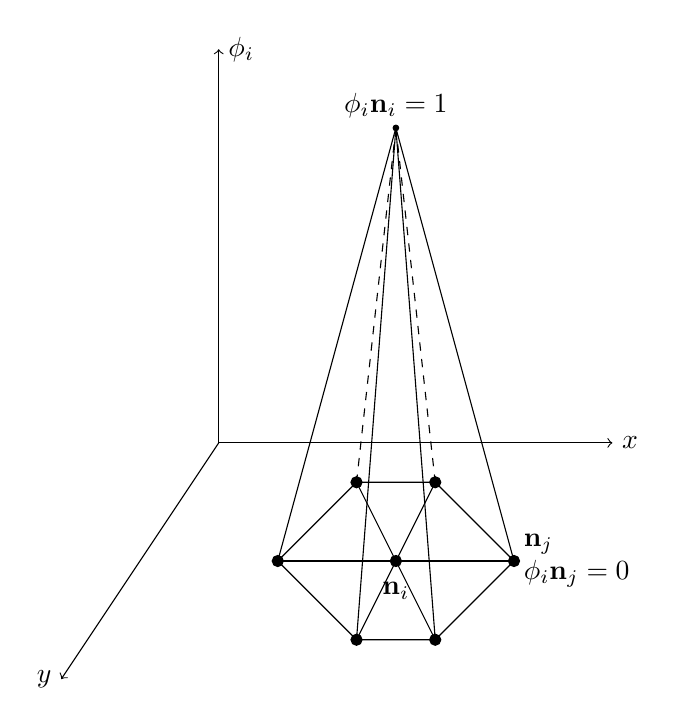
\begin{tikzpicture}
	\draw[->] (0,0) -- (0,5);
	\node[anchor=west] at (0,5) {$\phi_{i}$};
	\draw[->] (0,0) -- (5,0);
	\node[anchor=west] at (5,0) {$x$};
	\draw[->] (0,0) -- (-2,-3); 
	\node[anchor=east] at (-2,-3) {$y$}; %x,y,phi axis
	%draw "mesh part"
	\draw (0.75,-1.5) -- (1.75,-0.5) -- (2.75, -0.5) -- (3.75,-1.5) -- (2.75,-2.5) -- (1.75,-2.5) -- cycle;
	\draw (0.75,-1.5) -- (3.75,-1.5);
	\draw (1.75,-0.5) -- (2.75,-2.5);
	\draw (1.75,-2.5) -- (2.75,-0.5);
	\filldraw (0.75,-1.5) circle (2pt);
	\filldraw (1.75,-0.5) circle (2pt);
	\filldraw (2.75,-0.5) circle (2pt);
	\filldraw (3.75,-1.5) circle (2pt);
	\filldraw (2.75,-2.5) circle (2pt);
	\filldraw (1.75,-2.5) circle (2pt);
	\filldraw (2.25,-1.5) circle (2pt); %central node i
	\node[anchor=north] at (2.25,-1.65) {$\mathbf{n}_{i}$};
	%draw phi-lines to top
	\draw (2.25,4.0) -- (0.75,-1.5);
	\draw (2.25,4.0) -- (1.75,-2.5);
	\draw (2.25,4.0) -- (2.75,-2.5);
	\draw (2.25,4.0) -- (3.75,-1.5);
	\draw[dashed] (2.25,4.0) -- (1.75,-0.5);
	\draw[dashed] (2.25,4.0) -- (2.75,-0.5);
	%illustrate values of phi_i
	\filldraw (2.25,4.0) circle (1pt);
	\node[anchor=south] at (2.25,4.0) {$\phi_{i}\bracs{\mathbf{n}_{i}}=1$};
	\node[anchor=west, align=left] at (3.75,-1.5) {$\mathbf{n}_{j}$ \\ $\phi_{i}\bracs{\mathbf{n}_{j}}=0$};
	\end{tikzpicture}
	\caption{A typical choice for the basis functions $\phi_{i}$ is the 2-dimensional hat function. These functions are only non-zero on elements in $\eleSet$ which have $\mathbf{n}_{i}$ as a vertex. \label{fig:PhiIllustration}}
\end{figure}

For compactness we let $V = \femSolSpace$, and suppose we have a mesh $\eleSet$ for $\homDomain_{\epsilon, N}$ with $M$ nodes in a set $\nodeSet$ and mesh diameter $h$.
Let $u\in V$ be a solution to the boundary value problem \eref{HomProbFull} and $v\in V$ an arbitrary element of $V$.
To derive the weak formulation of \eref{HomProbMain}, we multiply through by $v$ and integrate over $\homDomain_{\epsilon, N}$ to obtain
\begin{align*}
	\int_{\homDomain_{\epsilon, N}}-v\laplacian u - \omega^{2}uv \ \mathrm{d}x = 0 &\quad \forall v\in V.
\end{align*}
Applying the Divergence Theorem to the term involving the Laplacian gives
\begin{align*}
	\int_{\homDomain_{\epsilon, N}}\grad u\cdot\grad v - \omega^{2}uv \ \mathrm{d}x + \int_{\othBoundary}v\bracs{\mathbf{n}\cdot\grad u}\ \mathrm{d}S = 0 &\quad \forall v\in V.
\end{align*}
Note here that only the integral over the non-periodic boundary appears, as the periodicity conditions are dealt with in the construction of the mesh.
By \eref{HomProbNeumann}, $\mathbf{n}\cdot\grad u=0$ on $\othBoundary$ and thus the surface integral is zero, and we arrive at
\begin{align}
	\int_{\Omega}\grad u\cdot\grad v - \omega^{2}uv \ \mathrm{d}x = 0 &\quad \forall v\in V\label{eq:FEMWeakForm}
\end{align}
which is the aforementioned weak formulation of \eref{HomProbFull}.
We also introduce the canonical notation
\begin{align*}
	a_{1}\bracs{u,v} &= \int_{\homDomain_{\epsilon, N}}\grad u\cdot\grad v \ \mathrm{d}x \\
	a_{2}\bracs{u,v} &= -\omega^{2}\int_{\homDomain_{\epsilon, N}} uv \ \mathrm{d}x,
\end{align*}
which defines two\footnote{Note that if we were not considering the eigenvalue problem, but rather had $\omega$ as a fixed parameter, it would be sufficient to only define a single bilinear form. However in order to solve the eigenvalue problem, IE for unknown $\omega$ and $u$, we are required to separate terms involving $\omega$ from terms that do not.} bilinear\footnote{The linearity properties are easily proved directly from the definitions of $a_{1}$ and $a_{2}$.} forms $a_{1},a_{2}:V\times V\rightarrow\reals$ whose sum comprises the left-hand-side of \eref{FEMWeakForm}.
The mesh $\eleSet$ comes equipped with a space $V_{h}\subset V$ over which we solve the weak formulation numerically\footnote{Note that linear interplants have trivial second derivative, and so are elements of $\Hp{2}{\homDomain_{\epsilon, N}}$ too.}.
Denote the finite element approximation to $u$ as $u_{h}$; and this approximate solution is the function $u_{h}\in V_{h}$ which solves
\begin{align} \label{eq:FEMWeakApprox}
	a_{1}\bracs{u_{h},v_{h}} = a_{2}\bracs{u_{h},v_{h}} &\quad \forall v_{h}\in V_{h}.
\end{align}
As $V_{h}$ is finite-dimensional and $a_{1}, a_{2}$ bilinear forms, it is sufficient to solve \eref{FEMWeakApprox} for all $\phi_{j}, j\in\mathset{1,...,M}$ rather than over all elements $v_{h}$ of $V_{h}$. 
We may also write $u_{h}$ as a sum of basis functions
\begin{align*}
	u_{h}\bracs{x} &= \sum_{\mathcal{I}}U_{i}\phi_{i}\bracs{x}
\end{align*}
for constants $U_{i}$.
Incorporating these insights into \eref{FEMWeakApprox} it can be seen that finding the FEM approximation amounts to solving
\begin{align} \label{eq:FEMWeakFinite}
	\sum_{i=1}^{M}a_{1}\bracs{\phi_{i},\phi_{j}}U_{i} &= \omega^{2}\sum_{i=1}^{M}a_{2}\bracs{\phi_{i},\phi_{j}}U_{i} \quad \forall j\in\mathset{1,...,M}
\end{align}
for the unknown constants $U_{i}$.
\eref{FEMWeakFinite} has a convenient matrix form $A^{(1)}\vU = \omega^{2}A^{(2)}\vU$ where the matrices $A^{(k)}$ (the stiffness matrices) have entries 
\begin{align*}
	A^{(1)} &= a_{1}\bracs{\phi_{i},\phi_{j}} = \int_{\homDomain_{\epsilon, N}}\grad\phi_{i}\cdot\grad\phi_{j} \ \mathrm{d}x \\
	A^{(2)} &= a_{2}\bracs{\phi_{i},\phi_{j}} = \int_{\homDomain_{\epsilon, N}}\phi_{i}\phi_{j} \ \mathrm{d}x
\end{align*}
Hence we may find eigenfrequencies $\omega^{2}$ and approximate eigenfunctions $u_{h}$ by finding solutions to the (generalised) eigenvalue equation
\begin{align} \label{eq:EvalEqn}
	A^{(1)}\vU &= \omega^{2}A^{(2)}\vU.
\end{align} 
Typically this is done using an iterative method, as direct solution is computationally expensive and unstable.
It is for this reason that we leave the problem in a form that does not involving matrix inverses (even though it will be shown that these exist as $A^{(1)},A^{(2)}$ are symmetric positive definite) which are computationally expensive, and become unstable when a matrix has a significant concentration of eigenvalues in an interval. \newline

When performing these numerics the domain was setup so that $\epsilon=\recip{10N}$; ensuring that $\epsilon N\rightarrow\recip{10}\in(0\infty)$, that the thin-structure setup was realisable without overlaps from different components, and placing us in a regime which has the problem from \sref{Graph2DNonClassicalKirchhoff} as its effective problem.
The FEM was implemented in Python 3.6 using software from FEniCS \cite{AlnaesBlechta2015a} to construct the stiffness matrices.
The eigenvalues in \eref{EvalEqn} were found using SciPy's eigenvalue solvers \cite{scipyReference}.

\section{Analysis} \label{sec:NumResultsFEM}
The choice of basis functions $\phi_{i}$ results in the stiffness matrices being sparse.
In particular, the products $\phi_{i}\phi_{j}$ and $\grad\phi_{i}\cdot\grad\phi_{j}$ are only non-zero when the nodes $\mathbf{n}_{i}$ and $\mathbf{n}_{j}$ are shared by an element\footnote{This is taken to include the case $i=j$.}.
This allows us to re-write the integrals over the whole domain $\homDomain_{\epsilon, N}$ as a sum of integrals over those elements $\tau\in\eleSet$ such that $\mathbf{n}_{i},\mathbf{n}_{j}$ are vertices of $\tau$, and hence provides this sparsity.
This is particularly useful when solving \eref{EvalEqn} numerically, as it allows for efficient matrix storage. 
However the approximation of the infinite-dimensional space $\femSolSpace$ by $V_{h}$ means that the FEM can never be used to obtain the entire (analytic) spectrum of the original operator.
As the matrices $A^{(1)},A^{(2)}$ are $M\times M$, the number of nodes places an upper limit on the number of eigenvalues we can find.
Refinements to the mesh (hence placement of additional nodes) allow deeper exploration of the spectrum, however this must be counterbalanced with the computational effort of finding the complete set of solutions to \eref{EvalEqn}. \newline

A well established bound for the error in the FEM is given in the Aubin-Nitsche theorem (see for example \cite{johnson2012numerical} for formal setup and proof).
For a mesh $\eleSet$ with diameter $h$, the error of the approximate solution $u_{h}$ in the $\lp{2}{\homDomain_{\epsilon, N}}$-norm is bounded by
\begin{align*}
	\norm{u - u_{h}}_{\lp{2}{\homDomain_{\epsilon, N}}} \leq Ch^{2}\norm{u}_{\Hp{2}{\homDomain_{\epsilon, N}}}
\end{align*}
provided that the mesh has some regularity\footnote{Precisely, the mesh $\eleSet$ must be shape-regular: there exists a constant $C>0$ such that $\frac{h_{\tau}^{2}}{\mu\bracs{\tau}}<C$ for all $\tau\in\eleSet$, where $\mu\bracs{\tau}$ denotes the area of the element $\tau$. Intuitively, this ensures that the elements cannot become arbitrarily long and thin.}.
In practice this bound is not particularly useful for choosing a mesh so that it produces an approximation correct to a certain error, as it requires knowledge of the solution $u$ and it's $\Hp{2}{\homDomain_{\epsilon, N}}$ norm.
However it does establish that a finer mesh (smaller $h$) reduces the error in the approximation, and the convergence to the solution $u$ (in the $\lp{2}{\homDomain_{\epsilon, N}}$-norm) is is quadratic. \newline

Trivially noting that the bilinear forms $a_{1}$ and $a_{2}$ are symmetric in their arguments, we have that $A^{(1)}$ and $A^{(2)}$ are symmetric.
Pursuing justification that the equation \eref{EvalEqn} has solutions, we prove positive definiteness of the stiffness matrix $A^{(1)}$.
First we prove that the bilinear forms $a_{1}$ is $V$-elliptic, that is that there exists a constant $c>0$ such that
\begin{align*}
	a_{1}\bracs{v,v} &\geq c_{1}\norm{v}_{V}.
\end{align*}
This is done by an application of the Poincar\'e inequality, $\norm{v}_{\lp{2}{\homDomain_{\epsilon, N}}}^{2}\leq C\norm{\grad v}_{\lp{2}{\homDomain_{\epsilon, N}}}^{2}$ and recognising that $a_{1}\bracs{v,v}=\norm{\grad v}_{\lp{2}{\homDomain_{\epsilon, N}}}^{2}$:
\begin{align*}
	\norm{v}_{V}^{2} &= \norm{\grad v}_{\lp{2}{\homDomain_{\epsilon, N}}}^{2} + \norm{\grad v}_{\lp{2}{\homDomain_{\epsilon, N}}}^{2} \\
	&\leq \bracs{C+1}\norm{\grad v}_{\lp{2}{\homDomain_{\epsilon, N}}}^{2} \\
	\Leftrightarrow \recip{C+1}\norm{v}_{V}^{2} &\leq \norm{\grad v}_{\lp{2}{\homDomain_{\epsilon, N}}}^{2} = a_{1}\bracs{v,v}.
\end{align*}
$\recip{C+1}>0$ as $C>0$, and as $v\in V$ was arbitrary, $a_{1}$ is $V$-elliptic.
Now for any vector $\mathbf{v}=\bracs{v_{1},...,v_{M}}^{\top}\neq\mathbf{0}$, we have that
\begin{align*}
	\mathbf{v}^{\top}A^{(1)}\mathbf{v} &= \sum_{i=1}^{M}\sum_{j=1}^{M}v_{i}v_{j}a_{1}\bracs{\phi_{i},\phi_{j}} \\
	&= a_{1}\bracs{\sum_{i=1}^{M}v_{i}\phi_{i},\sum_{j=1}^{M}v_{j}\phi_{j}} &\quad \text{(by bilinearity)}\\
	&= a_{1}\bracs{v_{h},v_{h}} \geq \norm{v_{h}}_{V} > 0
\end{align*}
where $v_{h}\in V_{h}\subset V$ is the element of $V_{h}$ with basis representation $v_{h}=\sum_{i=1}^{M}v_{i}\phi_{i}$.
Thus $A^{(1)}$ is positive definite.
Positive-definiteness of $A^{(2)}$ is more easily established, as for any $\mathbf{v}=\bracs{v_{1},...,v_{M}}^{\top}\neq\mathbf{0}$ and setting $v_{h}=\sum_{i=1}^{M}v_{i}\phi_{i}$ we have
\begin{align*}
	\mathbf{v}^{\top}A^{(2)}\mathbf{v} &= \sum_{i=1}^{M}\sum_{j=1}^{M}v_{i}v_{j}a_{2}\bracs{\phi_{i},\phi_{j}} \\
	&= a_{2}\bracs{\sum_{i=1}^{M}v_{i}\phi_{i},\sum_{j=1}^{M}v_{j}\phi_{j}} = a_{2}\bracs{v_{h},v_{h}} \\
	&= \int_{\homDomain_{\epsilon, N}}v_{h}^{2} \ \mathrm{d}x \\
	&>0;
\end{align*}
where the final inequality is strict because if $\mathbf{v}\neq\mathbf{0}$ the function $v_{h}$ cannot be the zero function as the $\phi_{i}$ form a basis of $V_{h}$, and hence the continuous and non-identically zero function $v_{h}^{2}\geq0$ cannot have zero integral over $\homDomain_{\epsilon, N}$.
This give us positive-definiteness of $A^{(2)}$ as well.
Now as $A^{(1)}$ is symmetric positive definite, so it is invertible with symmetric positive-definite inverse $\bracs{A^{(1)}}^{-1}$.
Hence solving \eref{EvalEqn} is equivalent to solving the eigenvalue equation
\begin{align} \label{eq:BetterEvalEqn}
	B\vU &= \omega^{2}\vU
\end{align}
where the matrix $B=\bracs{A^{(1)}}^{-1}A^{(2)}$ is the product of two symmetric positive-definite matrices.
Thus $B$ has positive eigenvalues\footnote{A short proof of this statement is as follows: Let $A_{1},A_{2}$ be symmetric positive-definite matrices. Then $A_{2}$ has symmetric positive-definite matrix square root $A_{2}^{\half}$. Hence we can express the product $A_{1}A_{2} = A_{2}^{-\half}\bracs{A_{2}^{\half}A_{1}A_{2}^{\half}}A_{2}^{\half}$, so $A_{1}A_{2}$ is similar to the symmetric positive-definite matrix $A_{2}^{\half}A_{1}A_{2}^{\half}$, hence has the same eigenvalues. The eigenvalues of a symmetric positive-definite matrix are strictly positive, hence so are the eigenvalues of $A_{1}A_{2}$.}. \newline

To conclude we present some numerical results for the spectra and associated eigenfunctions.
In order to demonstrate that the spectrum is becoming increasingly dense along the positive real line, we produce an integrated spectral density plot \fref{SpectralDensity} for the region $\bracs{0,2\pi}$.
\begin{figure}[b!]
	\centering
	\includegraphics[scale=0.75]{./Images/FEM_DensityOfStates.png}
	\caption{Integrated spectral density plot for various domains. The increasing density of the spectrum can be seen from visual inspection.\label{fig:SpectralDensity}}
\end{figure}
The integrated spectral density plot shows many eigenvalues lie below each value along the positive real line, normalised to the volume (in this case area) of $\homDomain_{\epsilon, N}$.
This plot provides us with information on how quickly the spectrum is \say{filling-up} the positive real line as $N$ increases - at the least the plots demonstrate that this \textit{is} happening.
This is to be expected given the analysis of \sref{Graph2DNonClassicalKirchhoff}; which is the effective problem for the thin-structure problem we consider here, and so we expect the spectrum to converge to (something close to) the band-gap spectrum obtained in that section.
We can see some evidence of this in \fref{SpectralDensity}; the integrated density remains constant over the interval $\omega\in\bracs{\pi,1.25\pi}$ which is consistent with the aforementioned analysis of the band-gap spectrum (each band terminating at $n\pi$).
If an analytic expression for the integrated density of states available, we could obtain the corresponding density of states for each spectrum which shows how the eigenvalues cluster about various points on the positive real line.
Unfortunately these plots are estimated from the numerical results to \eref{EvalEqn}, so instead we must turn to histograms to estimate the distribution along the positive real line of the eigenvalues.
Some examples of these are shown in \fref{NumericalSpectra} (these are in terms of the eigenfrequencies, which have been divided by $\pi$ to aid in visualising the spectrum). 
In these examples the smallest $1000$ eigenfrequencies were computed for each domain, and one can again notice that as $N$ increases the spectrum becomes increasingly dense.
The choice to only compute $1000$ eigenfrequencies was due to the available computer resources at the time; the system for $N=2,5,10$ had $4005,58096,446022$ nodes and $8046,104244,893621$ elements respectively, and so determining the full spectra was unfeasible\footnote{To work around this problem and take the analysis further, one may chose to examine the structure of the stiffness matrices to determine whether faster algorithms can be used.}.
Also plotted are some of the FEM solutions for the $N=2$ eigenfunctions (\fref{NumericalFunctions}), for visualisation.
Computationally there is no further difficulty in obtaining the eigenfunctions having obtained the eigenvalues as they are computed in the same algorithm, however higher values of $N$ result in it being difficult to see the variation of the eigenfunctions along the \say{tubes}.
\begin{figure}[h!]
	\centering
	\subfigure[Smallest $1000$ eigenfrequencies for the $N=2$ domain.]{
		\centering
		\includegraphics[scale=0.45]{./Images/HistN2full.png}
	}
	\quad
	\subfigure[Smallest $1000$ eigenfrequencies for the $N=5$ domain.]{
		\centering
		\includegraphics[scale=0.45]{./Images/HistN5full.png}
	}
	\quad
	\subfigure[Smallest $1000$ eigenfrequencies for the $N=10$ domain.]{
		\centering
		\includegraphics[scale=0.45]{./Images/HistN10.png}
	}
	\caption{The smallest $1000$ eigenfrequencies for various domains. Note that as $N$ increases the spectrum becomes increasingly dense; the $1000^{\mathrm{th}}$ eigenfrequency in the $N=10$ problem is approximately $6$ times smaller than it's $N=2$ counterpart.  \label{fig:NumericalSpectra}}
\end{figure}
\begin{figure}[h!]
	\centering
	\subfigure[The eigenfunction for the eigenfrequency $\omega = 0.9736174525997192$ in the $N=2$ domain ($3^{\mathrm{rd}}$ smallest eigenfrequency).]{
		\centering
		\includegraphics[scale=0.5]{./Images/FEM_Solution_N2_3eval.png}
	}
	\quad
	\subfigure[The eigenfunction for the eigenfrequency $\omega = 25.37447775539648$ in the $N=2$ domain ($125^{\mathrm{th}}$ smallest eigenfrequency).]{
		\centering
		\includegraphics[scale=0.5]{./Images/FEM_Solution_N2_125eval.png}
	}
	\caption{Visualisation of the eigenfunctions corresponding to the $3^{\mathrm{rd}}$ and  $125^{\mathrm{th}}$ eigenfrequencies, in the $N=2$ domain. Note that the higher-$\omega$ eigenfunction varies more rapidly in the non-zero areas than it's counterpart. \label{fig:NumericalFunctions}}
\end{figure}
